% !TeX root = ../relazione.tex

\chapter{Progettazione}


\section{Architettura} \label{sec:architettura}
Il progetto è basato su una architettura 3-tier \cite{wiki:3-tier-architecture},
ovvero è suddiviso in 3 diversi moduli sviluppati separatamente e dedicati alla
gestione dei dati (\textbf{Data tier}), alla logica funzionale (Logic o
\textbf{Application tier}) e all'interfaccia utente (\textbf{Presentation tier});
questi comunicano e scambiano dati tra loro con un approccio client-server.

Con questa architettura è possibile raggiungere un buon livello di scalabilità
e modularità, evitando di includere la logica dell’applicazione sia a livello del
server che lato client (modello 2-tier).

\begin{figure}[ht]
	\centering
	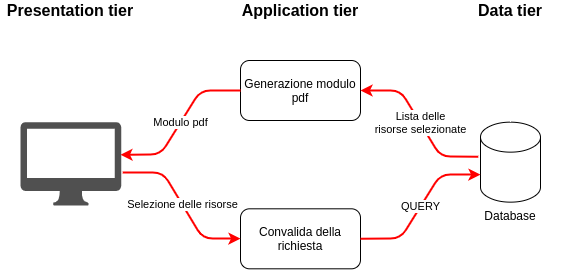
\includegraphics[width=0.8\textwidth]{assets/diagrams/3-tier-resources-selection.png}
	\caption{Selezione delle risorse con l'architettura 3-tier}
	\label{fig:3-tier-resources-selection}
\end{figure}

Il terzo livello software inserito nel mezzo contiene la maggior parte della logica
e si posiziona ad un livello intermedio in modo da essere disponibile ad ogni
servizio del sistema. Nel momento in cui è necessario cambiare un componente di
logica dell’applicazione è sufficiente modificare solo un "mattoncino" specifico del
livello intermedio.
Ognuno dei tre livelli architetturali è associato ad un specifica categoria logica:
\begin{itemize}
	\item Il Presentation tier sarà la UI (User Interface) dei servizi per l’utente,
	garantendogli la possibilità di interagire con gli altri livelli tramite
	un'interfaccia grafica, in maniera trasparente
	\item L'Application tier si occupa della parte applicativa e logica,
	include l’esecuzione di applicazioni, la logica che si occupa della convalida
	dei dati e delle richieste/risposte nella comunicazione fra i processi degli
	altri livelli
	\item Il Data tier include i servizi che gestiscono il database; che forniscono
	i dati necessari al completamento delle richieste del livello Logico. In questo
	caso la logica del server interagisce con la gestione, l’accesso e la sicurezza
	dei dati
\end{itemize}
Tra i vantaggi di questa architettura possiamo includere la distribuzione e la
riusabilità del codice, in quanto tutte le logiche che vengono utilizzate dagli
utenti finali sono nel server intermedio. Un'altra caratteristica è che questa
separazione tra l'interfaccia utente, la logica ed i dati permette una maggiore
flessibilità nello sviluppo di nuove funzionalità; ad esempio dato che le
componenti server e logiche sono già testate, lo sviluppo di un nuovo componente
nella UI sarà più rapido e con una fase di test più breve. In pratica un
aggiornamento, il fix di un bug o l'implementazione di una nuova funzionalità di
un singolo livello applicativo ha un impatto minimo sugli altri.

L'approccio si riflette anche nella gerarchia delle competenze, in quanto gli
eventuali team di sviluppo si possono separare in diverse tipologie per
specializzarsi negli ambiti relativi ai 3 livelli dell'architettura: il front-end,
il back-end ed il data-end. La scalabilità è un aspetto fondamentale di questa
architettura in quanto separando i diversi livelli ognuno può scalare in termini
di capacità e potenza indipendentemente dagli altri. Per esempio se stiamo ricevendo
un numero elevato di richieste web che non si stanno traducendo in un carico
direttamente proporzionale in richieste computazionali che caricano le applicazioni,
possiamo scalare solo questo livello.

\section{Sessione utente}
Trattandosi di una piattaforma web le cui funzionalità sono pensate per essere
accessibili solo a seguito di autenticazione, la gestione della sessione utente
ne è una parte molto importante. Una sessione rappresenta infatti la possibilità
che un utente possa usufruire di un servizio in maniera continua, senza doversi
autenticare ad ogni operazione che necessita di verificare che si sia in possesso
di un account valido o che si abbiano permessi sufficienti.

\paragraph{Approccio basato su token}
L'approccio utilizzato è quello basato su \textbf{token}, per cui a seguito
di ogni autenticazione deve essere generato e associato all'utente un codice
univoco, volto a verificare la sessione. Questo codice, detto \textit{token}, è
definito come valido per un breve periodo di tempo, ma viene "rinnovato" ad ogni
richiesta effettuata dal client verso l'Application tier, così da garantire la
continuità della sessione, fino alla scadenza o al logout esplicito da parte
dell'utente.
Per ogni richiesta effettuate viene quindi verificato che l'utente sia autenticato
e che sia autorizzato ad effettuare eventuali operazioni riservate (ad esempio
accedere al pannello di amministrazione).


\section{Diagramma ER}

Il diagramma in \autoref{fig:er-diagram} è stato progettato con MySQL WorkBench
\cite{workbench:9-EER} ed utilizza la notazione \textit{crow's foot}
\cite{wiki:crows-foot}, più orientata all'implementazione, in cui le relazioni
sono rappresentate da linee che collegano le entità e la cui cardinalità è
espressa tramite i simboli presenti alle estremità (\autoref{fig:crows-foot-notation}).

\begin{figure}[ht]
	\centering
	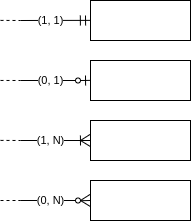
\includegraphics[width=0.4\textwidth]{assets/diagrams/crows-foot-notation.png}
	\cprotect\caption{notazione \textit{crow's foot}}
	\label{fig:crows-foot-notation}
\end{figure}

\paragraph{}
Le tipologie di utenti sono unificate nella tabella \textit{user} e la
suddivisione è gestita tramite la tabella \textit{user\_type}. Le relazioni di
\textit{user} con \textit{submission\_change} e \textit{download\_link}
rappresentano le operazioni effettuate dagli utenti gestori/amministratori per
quanto riguarda il cambio stato e la generazione di link per scaricare le risorse.

\begin{figure}[ht]
	\centering
	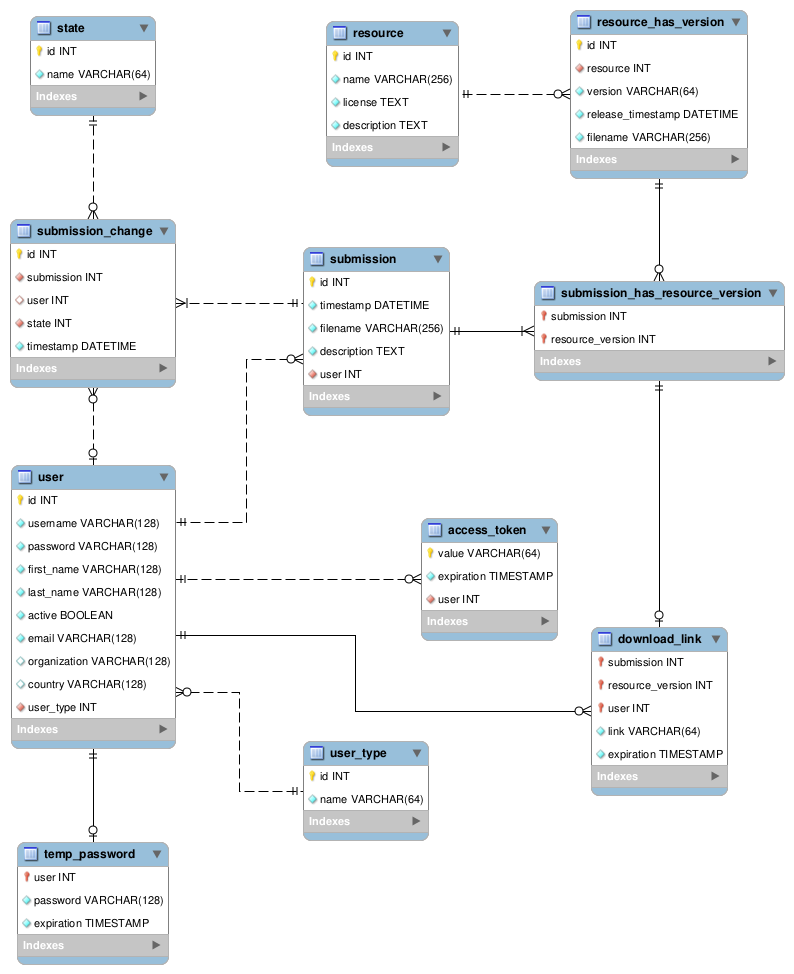
\includegraphics[width=\textwidth]{assets/diagrams/db-er-diagram.png}
	\caption{Diagramma ER}
	\label{fig:er-diagram}
\end{figure}